\documentclass{proyectotesis}

\usepackage[backend=biber,natbib=true,sorting=none,style=numeric-comp, maxcitenames=2, url=false, isbn=false]{biblatex}
\usepackage{csquotes}
\DefineBibliographyStrings{spanish}{andothers={et al.}}
\AtEveryBibitem{\clearfield{note}}
\addbibresource{refs.bib}

%%%%%%%%%%%%%%%%%%%%%%%%%%%%%%%%%%%%%%%%%%%
%%%%%%%%%%%%%%%%%%%%%%%%%%%%%%%%%%%%%%%%%%%
%%%%%%%%%%%%%%%%%%%%%%%%%%%%%%%%%%%%%%%%%%%

\title{Detección de comunidades y polarización en redes legislativas}
\author{Benjamín Matías Ortiz Edwards}
\pronom{el}
\postgrado[Magíster]{en Ciencias con mención en Física.}
%\directora{}
%\director{}
\directores{Dra. Denisse Pastén y Dr. Víctor Muñoz}
%\codirector{}
\duracion{Primer y segundo semestre 2022.}
\lugar{Grupo Planets (www.planets.cl), Departamento de Física, Facultad de Ciencias, Universidad de Chile.}
\direccion{Las Palmeras 3425, Ñuñoa, Santiago, Chile. \\Dirección Postal: Casilla 653, Santiago, Chile. Fono: (56-2) 2978 7276.}

%%%%%%%%%%%%%%%%%%%%%%%%%%%%%%%%%%%%%%%%%%%
%%%%%%%%%%%%%%%%%%%%%%%%%%%%%%%%%%%%%%%%%%%
%%%%%%%%%%%%%%%%%%%%%%%%%%%%%%%%%%%%%%%%%%%

\nacimiento{10 de febrero, 1997}
\RUN{19.359.906-0}
\telefono{(+56\;9)\:8656\;0757}
\email{bedw@bedw.me}

\begin{document}

\maketitlepage
\makepersonalinfo

%%%%%%%%%%%%%%%%%%%%%%%%%%%%%%%%%%%%%%%%%%%
%%%%%%%%%%%%%%%%%%%%%%%%%%%%%%%%%%%%%%%%%%%
\subsection{Educación}
\begin{cvlist}{}
\item[\textbf{Educación Superiror}] 
\item[\textbf{2015 - 2020}] Licenciatura en Ciencias con mención en Física, Universidad de Chile.
\item[\bf Educación Escolar]
\item[\textbf{2010 - 2014}]  Enseñanza Básica y Media, Colegio Compañia de María Seminario.
\end{cvlist}

\subsection{Experiencia Profesional}
\begin{cvlist}{}
\item[\textbf{2020}]   \textbf{Ayudante},  Métodos de la Física Matemática II, Departamento de Física, Facultad de Ciencias, Universidad de Chile, Segundo Semestre.
\item[\textbf{2021}]   \textbf{Ayudante},  Métodos de la Física Matemática II, Departamento de Física, Facultad de Ciencias, Universidad de Chile, Segundo Semestre.
\item[\textbf{2019}]  \textbf{Practicante}, "Practicas de Verano", DFC-DFI, Universidad de Chile.   
\item[\textbf{2021 - Presente}] \textbf{Programador analista}, Centro de Inteligencia Territorial, Universidad Adolfo Ibañez. 

\end{cvlist}

\subsection{Presentaciones a Congresos}

\begin{cvlist}{}
\item[\textbf{2020}] \textbf{Ortiz Edwards, B.}, Pastén, D., y Muñoz, P. S. A complex network approach on the analysis of the Chilean presidential elections, using Twitter Data, {\it Complex Networks 2019}, Lisboa, Portugal, 10-12 de diciembre.

\end{cvlist}

\newpage

\section{Exposición General del Proyecto}
\subsection{Resumen}

\subsection{Introducción}
Las \textbf{redes complejas} son muy útiles para caracterizar sistemas con muchos elementos que interactúan entre sí Estas nos permiten modelar distintos sistemas mediante una representación de grafos, con nodos y conexiones, para luego obtener distintas propiedades del sistema a partir de métricas, o propiedades estadísticas o topológicas de la red. Estas se han utilizado en diversas disciplinas, como: el estudio de redes sociales~\cite{newman_structure_2003, cantwell_friendship_2021}, redes en internet~\cite{newman_structure_2003}, redes biológicas~\cite{newman_structure_2003, da_fontoura_costa_complex_2008}; en epidemiología~\cite{karrer_competing_2011}, ahora más recientemente identificando agentes difusores de COVID~\cite{montes-orozco_identification_2020}; y por otro lado, en la categorización de subtormentas magnetosféricas~\cite{dods_network_2015}, por mencionar algunos ejemplos.\\

Si bien hay diversos trabajos que vinculan redes con física --por ejemplo estudiando la mecánica estadística de redes complejas~\cite{albert_statistical_2001, pastor-satorras_statistical_2003}, o abordando la dinámica de opiniones en redes, con modelos sociofísicos~\cite{suchecki_conservation_2005, castellano_statistical_2009}-- en este proyecto queremos abordar un problema en particular: la \textbf{detección de comunidades}, la cual consiste en identificar clusters o comunidades de nodos a partir de las conexiones que tienen entre sí, y de que tan intensas sean estas.\\

%Un area en donde sin duda han tenido un gran impacto son las ciencias sociales. En estas, las redes permiten estudiar las relaciones entre personas (o grupos de personas) como conexiones, pudiendo estas ser de diversos tipos. Por ejemplo: relaciones de amistad, sexuales, de trabajo, políticas, entre otras.\\

Para detectar comunidades hay diversos algoritmos, pero sin duda los mas utilizados son aquellos que maximizan la modularidad ($Q$)~\cite{newman_fast_2004, clauset_finding_2004, duch_community_2005, blondel_fast_2008, arab_modularity_2012, chen_community_2014}. Esta cantidad fue definida inicialmente por \citet{newman_finding_2004} y da cuenta de que tan ``modular'' es una red según una partición de comunidades --entendiendo una partición de comunidades como el conjunto de etiquetas que indican las comunidades asignadas a cada nodo en la red. Como se mencionó anteriormente, muchos algoritmos maximizan esta medida para detectar comunidades. En términos sencillos, estos prueban distintas comunidades y evalúan la modularidad. Luego, la partición de comunidades que maximiza la modularidad es el \textit{output} del algoritmo.\\

Sin embargo, pese a que este problema se suele abordar con un enfoque casi netamente matemático, hay autores que lo relacionan con principios de \textbf{mecánica estadística}. Reichardt y Bornholdt desarrollaron el algoritmo llamado ``Spin-Glass'' para detectar comunidades ~\cite{reichardt_statistical_2006}, el cual aborda el problema definiendo un hamiltoniano que debe minimizarse para obtener la partición de comunidades óptima. La idea detrás del algoritmo es, en un vidrio de \textit{spin}, hacer el símil entre las partículas con mismo \textit{spin}, con nodos de una misma comunidad, definiendo las interacciones \textit{spin-spin} a partir de las conexiones de la red. Los autores además demostraron que la minimización de la energía (del hamiltoniano) es equivalente a la maximización de la modularidad.\\

Una aplicación concreta para la para la detección de comunidades es el estudio de polarización (política) en redes legislativas --en donde se estudian las relaciones entre los miembros de  parlamentos de distintos países, usando análisis de redes.\\

Como contexto, la mayoría trabajos de redes legislativas~\cite{neal_sign_2020, marenco_time_2020, intal_dissent_2021, schoch_legislators_2020, aleman_explaining_2013, zhang_community_2007, fowler_connecting_2007, porter_network_2005, andris_rise_2015, briatte_network_2016, le_foulon_moran_cooperation_2020}
tienen más o menos en común la forma en que crean las redes. En estas los \textbf{parlamentarios se representan como nodos, y las relaciones entre ellos como conexiones}, las cuales generalmente tienen pesos, indicando que tan intensa en la relación. Qué se considera como relaciones entre los parlamentarios varía de trabajo en trabajo, pero los más común es que las relaciones indiquen patrocinio en conjunto a las propuestas de ley~\cite{neal_sign_2020, zhang_community_2007, le_foulon_moran_cooperation_2020,fowler_connecting_2007}, co-participación en comisiones~\cite{porter_network_2005}, o la coordinación (o descoordinación) de los parlamentarios al momento de votar~\cite{andris_rise_2015, marenco_time_2020, schoch_legislators_2020, intal_dissent_2021}.\\

Para estudiar la polarización de en una red legislativa es necesario detectar comunidades en ella. Luego, la red se considera polarizada cuando los nodos de una misma comunidad tienen interacciones más fuertes entre sí, mientras que más débiles (o nulas) con los nodos de distintas comunidades. Esta concepción de polarización es llamada ``polarización débil'' por \citet{neal_sign_2020}. Sin embargo, en su trabajo también propone un segundo tipo de polarización, que denomina ``polarización fuerte''. Esta consiste en que, además de haber muchas conexiones (e intensas) entre los nodos de una misma comunidad, entre nodos de comunidades diferentes existan conexiones pero de peso negativo. Una manera de interpretar esto es considerar las conexiones de peso positivo como fuerzas atractivas, y las de peso negativo repulsivas --de este modo habrán individuos que se ``acercan'', mientras otros se ``alejan''.\\

Finalmente, para cuantificar la polarización, varios autores usan la misma medida de modularidad como un indicador de esto --considerando que mientras más alta sea la modularidad, la red está más polarizada. Sin embargo, esto solo servirá para medir polarización débil, ya que la modularidad como tal no está definida para conexiones con pesos negativos. Ante esto, \citet{neal_sign_2020} propone usar el índice de triángulo~\cite{aref_measuring_2018} para cuantificar la polarización fuerte. Este índice indica que tan balanceada se encuentra la red, entendiendo balance como la ``proporción'' entre conexiones de peso positivo y negativo en la red.\\

Este proyecto busca usar estas ideas y aplicarlas en el estudio de la polarización de la Cámara de Diputados de Chile, a partir de las interacciones entre los miembros de esta. La motivación principal es que en la literatura, si bien encontramos estudios sobre la Cámara de Diputados Chilena con análisis de redes, estos solo abarcan periodos legislativos desde el inicio de la década de los 2000 hasta el 2017~\cite{aleman_explaining_2013, le_foulon_moran_cooperation_2020}. Sin embargo, desde entonces la política Chilena ha sufrido cambios significativos: a partir del 2018 ingresan nuevas fuerzas políticas al parlamento, y en medio del periodo legislativo que inicia ese año ocurre un estallido social y una pandemia.\\

Ahora, nos preguntamos: ¿Es posible medir la polarización política de la Cámara de de Diputados de Chile desde el 2018 en adelante, usando análisis de redes? De ser posible, ¿Esta polarización es de tipo débil o fuerte? Por otro lado, ¿Habrá un método basado en mecánica estadística para detectar comunidades, de forma similar al planteado por \citet{reichardt_statistical_2006},  que sea equivalente a la maximización del índice de triángulo, para así dar cuenta de la polarización fuerte? %Por último, también, ¿Es el Índice del triángulo la forma más optima de cuantificar la polarización fuerte?

\subsection{Objetivos}

%Se busca desarrollar un algoritmo que permita detectar comunidades en redes con pesos negativos, a partir de principios de mecánica estadística, considerando su posterior aplicación en la 
En el contexto del estudio de interacciones entre los miembros de la Cámara de Diputados de Chile, se busca elaborar un algoritmo que nos permita detectar comunidades en una red con pesos negativos, y posteriormente cuantificar la polarización de la Cámara, a partir de principios de mecánica estadística.

%También evaluaremos los algoritmos de detección de comunidades basados en la maximización de modularidad como una medida ``óptima'' de polarización política. Para ello se propone comparar los valores de modularidad y , con el índice de triángulo, al considerar interacciones negativas (repulsivas). 
%También se busca desarrollar una medida de polarización basada en mecánica estadística, basándonos en trabajos similares.

\subsubsection*{Objetivos Específicos}
\begin{itemize}
\item    {\bf Análisis de Redes Complejas.} Caracterizar la interacción entre miembros de la Cámara de Diputados de Chile, por medio de la representación del sistema como red compleja, a partir de los datos públicos de las votaciones en sala.

\item{\bf Comparación entre la modularidad y el índice del triángulo.} Con la red construida se propone detectar comunidades usando el algoritmo ``Spín-Glass''~\cite{reichardt_statistical_2006}, para luego medir la modularidad~\cite{newman_finding_2004}, y comparar esta cantidad con el índice de triángulo~\cite{aref_measuring_2018}. El propósito de esto es identificar nociones de polarización débil o fuerte con las herramientas que en este momento tenemos a disposición.

\item {\bf Desarrollo de nuevo algoritmo de detección de comunidades, basada en mecánica estadística.} De forma similar a lo realizado po \citet{reichardt_statistical_2006}, se busca crear algoritmo para detectar comunidades en una red con conexiones negativas, basado en la minimización de un hamiltoniano, pero que se relacione con la maximización del índice de triangulo para dar cuenta de la polarización fuerte en un red legislativa.

\end{itemize}

\subsection{Metodología}
\subsubsection{Análisis de Redes Complejas.}
Se busca caracterizar la interacción entre miembros de la Cámara de Diputados de Chile por medio de la representación del sistema como red (a partir de los datos públicos de las votaciones en Sala), siguiendo una metodología basada en lo realizado en trabajos anteriores~\cite{andris_rise_2015, marenco_time_2020, schoch_legislators_2020, intal_dissent_2021}. 

En términos simples, cada nodo de la red representará un parlamentario, y estos tendrán conexiones según la coordinación (o descoordinación) de los representantes al momento de votar en Sala.\\

Para una votación en Sala $k$, representaremos los votos mediante el vector 
\begin{equation}
    v^k = \{u_1,\dots,u_n\}
\end{equation}
con $u_i$ la opción que el o la parlamentaria $i$ votó. Esta será 1 si el voto fue a favor, -1 si fue en contra y 0 en caso de abstención o ausencia.

Realizando el producto externo de $v^k$ consigo mismo, se obtiene la matriz $M^k$ que representa la coordinación de los parlamentarios en la votación $k$. De esta forma la coordenada $M^k_{ij}$ será 1 si los parlamentarios $i$ y $j$ votaron lo mismo, -1 si votaron opciones opuestas, y 0 si alguno se abstuvo o estuvo ausente. Entonces, ahora, para $m$ votaciones, sumamos las matrices $M^k$.
\begin{equation}
    A_{ij} = \sum_k^m M^k_{ij} \label{adj}
\end{equation}
Con esta matriz ya podemos crear la red. Si una coordenada $A_{ij}\neq 0$ entonces creamos una conexión entre los nodos $i$ y $j$ , y con una peso igual a $A_{ij}$. Para los casos $A_{ij} = 0$, simplemente no se crea ninguna conexión entre los nodos $i$ y $j$.\\

Por otro lado, la modularidad~\cite{newman_finding_2004} se define por
\begin{equation}
    Q = \frac{1}{2m}\sum_{ij} \left( A_{ij} - \frac{k_i k_j}{2m}  \right) \delta(\sigma_i,\sigma_j) \label{mod}
,\end{equation}
con $k_i$ la suma de los pesos de las conexiones del nodo $i$, $m = \frac{1}{2} \sum_i k_i$. También tenemos $\sigma_i$ que indíca a que comunidad pertenece el nodo $i$, y $\delta(\sigma_i,\sigma_j)$ se define de tal forma que es 1 si los nodos $i$ y $j$ pertenecen a la misma comunidad, o 0 en caso contrario.\\

Queda por definir cuantas y cuales votaciones se considerarán para armar la red. Se plantea también la idea de armar varias redes a partir de votaciones ocurridas en periodos o intervalos de tiempo distintos. Al agregar la dimensión temporal podemos un estudio longitudinal de la polarización, y analizar como esta cambia (o no) en el tiempo, por ejemplo.

\subsubsection{Comparación entre la modularidad y el índice de triángulo} 
Luego de crear la red a partir de la matriz de adjacencia de la ecuación \eqref{adj}, se busca medir la modularidad y el índice de triángulo para compararlos. Para ello se propone momentáneamente ``ignorar'' las conexiones negativas, remplazando todas las entradas de $A_{kl} < 0$. Ahora, con esta red de solo conexiones de peso positivo, detectaremos comunidades con el método ``Spin-Glass''~\cite{reichardt_statistical_2006} y con la partición de comunidades resultante, a la red le calculamos la modularidad. \\

Posteriormente, con la misma partición de comunidades resultante del proceso anterior, pero ahora sí considerando las conexiones de peso negativo, a la red se le medirá el índice de triángulo. \\

Luego, esta medida se comparará con la modularidad ya calculada. Este proceso podrá ser complementado con un análisis visual de la red, en el cual se aprecie de forma gráfica el peso de las conexiones (como el largo de los segmentos) y que diferencie las de peso negativo con las de peso positivo.\\

Para comprender la definición del índice de triángulo~\cite{aref_measuring_2018} primero introduciremos lo que son los ciclos balanceados y no balanceados~\cite{aref_measuring_2018}.\\

Un ciclo, es decir, una secuencia de nodos conectados en la que el primer nodo es igual al último, será balanceado si el producto de sus pesos de sus conexiones es mayor a cero. En caso de que sea menor a cero el ciclo se considera no balanceado.\\

Ahora, $O_k^+$ dará cuenta de la cantidad de ciclos balanceados de $k$ nodos, mientras que $O_k^-$ la cantidad de ciclos de $k$ nodos no balanceados. Además, $O_k = O_k^+ + O_k^-$ será la cantidad total de ciclos de $k$ nodos. Finalmente, el Índice del triángulo se define como
\begin{equation}
    T(G) = \frac{O_3^+}{O_3},
\end{equation}

\subsubsection{Desarrollo de nuevo algoritmo de detección de comunidades, basada en mecánica estadística} 
Como se mencionó anteriormente, Reichardt y Bornholdt desarrollaron el algoritmo ``Spin-Glass'' para detectar comunidades~\cite{reichardt_statistical_2006}. El principio detrás de este consiste en la minimización de un hamiltoniano. También demostraron que minimizar tal hamiltoniano es equivalente a maximizar la modularidad bajo ciertas condiciones.

Al momento de desarrollar el Hamiltoniano, los autores lo abordaron de la siguiente manera
\begin{align}
\begin{split}
    \mathcal{H}(\{\sigma\}) = &- \underbrace{\sum_{i\neq j} a_{ij}A_{ij}\delta(\sigma_i,\sigma_j)}_{(a)} + \underbrace{\sum_{i\neq j} b_{ij}(1 - A_{ij})\delta(\sigma_i,\sigma_j)}_{(b)} \\
                              &+ \underbrace{\sum_{i\neq j} c_{ij} A_{ij}[1 - \delta(\sigma_i,\sigma_j)] }_{(c)} - \underbrace{\sum_{i\neq j} d_{ij} (1-A_{ij})[1 - \delta(\sigma_i,\sigma_j)]}_{(d)}
\end{split}
\label{Ham}
\end{align}
En \eqref{Ham}, $\sigma$ representa la partición de comunidades, donde, en concreto $\sigma_i$ indica a que comunidad pertenece el nodo $i$. Luego $\delta(\sigma_i,\sigma_j)$ se define de tal forma que es 1 si los nodos $i$ y $j$ pertenecen a la misma comunidad, o 0 en caso contrario.

Notemos también lo siguiente. El término $(a)$ corresponde a las conexiones entre nodos de una misma comunidad, y $(d)$ las desconexiones entre nodos de distintas comunidades. Por otro lade tendremos que el término  $(b)$ representa las desconexiones entre nodos de una misma comunidad, mientras que $(c)$ las conexiones entre nodos de distintas comunidades.\\

Notando el signo antes de cada uno de estos términos podemos apreciar como este tipo de hamiltoniano busca ``premiar'' a las conexiones intra-comunidades y a las desconexiones inter-comunidades, al mismo tiempo que ``penaliza'' las conexiones inter-comunidades o la ausencia de conexiones entre nodos de una misma comunidad.
\\

Siguiendo una lógica similar a lo recién planteado, se busca desarrollar un hamiltoniano que nos permita detectar comunidades, ahora, en una red con conexiones de peso negativo, y cuya minimización sea equivalente a la maximización del índice de triángulo.

\subsection{Trabajo adelantado}
Anteriormente ya hemos realizamos un análisis de redes a la Cámara de Diputados. Para esto se usaron datos públicos de las votaciones en Sala ocurridas entre Marzo de 2018 y Diciembre 2020, los cuales están disponibles en línea mediante una API de libre acceso.\\ 

Se construyeron varias redes, y la manera en que se cada construyó cada  una fue la siguiente. Para una votación, si dos parlamentarios votan la misma opción (a favor, en contra o  abstención), se crea una conexión entre ambos parlamentarios, y en caso contrario, no se crea ninguna conexión. Ahora, para varias votaciones el procedimiento es similar, sin embargo en este caso a las conexiones se les asignó un peso, el cual fue igual a la cantidad de veces que cada par de parlamentarios coincidió al momento de votar en las votaciones consideradas.

De esta manera se crearon redes mensuales, es decir considerando las votaciones ocurridas en el periodo de un mes, para cada mes.

Notemos que la diferencia de esto con lo propuesto el la sección de Metodología, es que acá no consideramos las conexiones con peso negativo cuando los parlamentarios votan opciones opuestas.\\

Luego, a cada a red mensual se le detectaron comunidades usando 2 algoritmos distintos distintos (Louvain~\cite{blondel_fast_2008} y Spin-Glass~\cite{reichardt_statistical_2006}) y se les midió la modularidad con cada una de la particiones de comunidades obtenidas. En la figura \ref{modfig} podemos ver como varia la modularidad en el tiempo, mientras que en la figura \ref{N} vemos el número de comunidades detectadas.\\
\begin{figure}[h!]
    \centering
    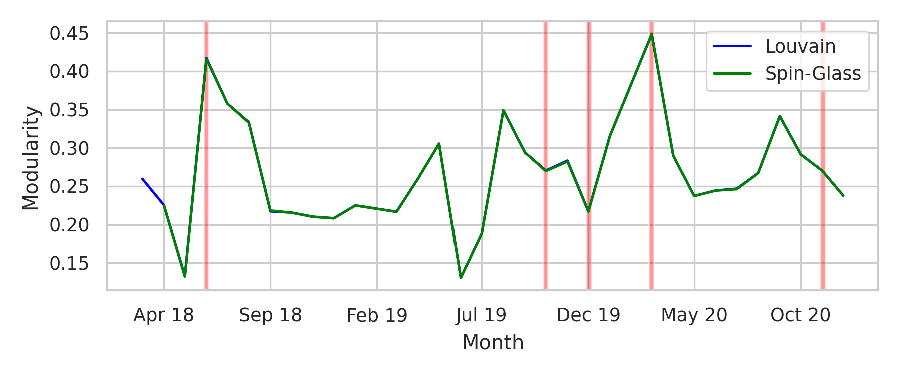
\includegraphics[width=0.95\linewidth]{mod.pdf} 
    \vspace{-5mm}
    \caption{Modularidad obtenida luego de detectar comunidades con cada algoritmo, en el tiempo. Las franjas rojas representan meses en que ocurrieron hitos políticos de la Tabla \ref{hp}.}
    \label{modfig}
\end{figure}
\begin{figure}[h!]
    \centering
    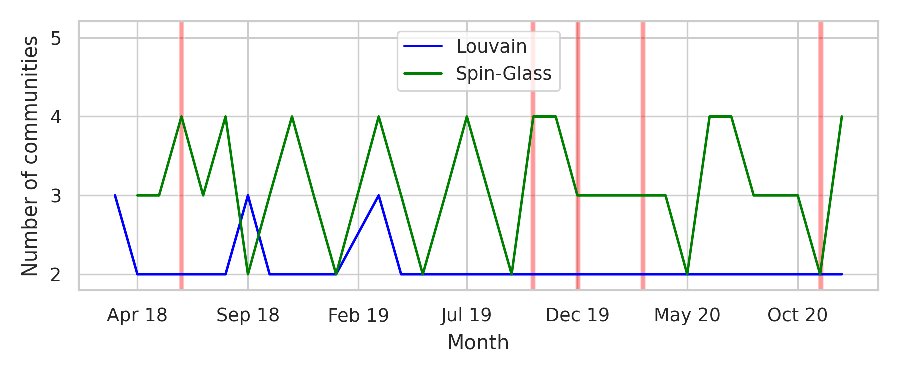
\includegraphics[width=0.95\linewidth]{N.pdf} 
    \vspace{-5mm}
    \caption{Numero de comunidades detectada por cada algoritmo, en el tiempo. Las franjas rojas representan meses en que ocurrieron hitos políticos. Las franjas rojas representan meses en que ocurrieron hitos políticos de la Tabla \ref{hp}.}
    \label{N}
\end{figure}

\renewcommand{\tablename}{Tabla}

\begin{table}[ht!]
    \centering
    \caption{Meses en los que ocurrieron hitos políticos relevantes}
    \label{hp} 
    \begin{tabular}{r|l}
    Mes & Hito Político.\\
    \hline
    Junio 2018 & Diputados presenta proyecto de Ley de Aborto Libre.\\
    Octubre 2019 & Inicia el estallido social.\\
    Diciembre 2019 & Se ingresa al parlamento el proyecto de ley que permite el cambio de constitución.\\
    Marzo 2020 & Se aprueba la paridad para la Convención Constitucional.\\
    Octubre 2020 & Se aprueban los escaños reservados para la Convención Constitucional.
    \end{tabular}
\end{table}


Primero notamos que los 2 métodos resultaron prácticamente idénticos para los efectos de calcular la modularidad, habiendo mayores diferencias en en el número de comunidades detectadas. Las figuras sugieren que el método Sping-Glass es mucho más sensible para la detección de comunidades, ya que este número fluctúa mucho más que para el otro algoritmo. También se puedo apreciar que los peaks más altos de modularidad (Sep ’18 y Marzo ’20) coinciden con una baja del numero de comunidades respecto a los meses anteriores.

Por otro lado, estos dos meses fueron bastante activos en términos legislativos. Desde Diciembre de 2020 hasta Marzo de 2020 el parlamento aprueba el cambio el cambio constitucional que permitiría el nuevo proceso constituyente, y también discute aspectos relevantes de este, como la paridad de genero, siendo esta aprobada en marzo. Por otro lado, durante Junio de 2018, el parlamento intenta responder a las demandas del movimiento feminista que desde Mayo de ese año ya había generado grandes manifestaciones a lo largo de todo Chile. En esta ocasión, un grupo de parlamentarios presenta un proyecto de aborto libre, lo que generó harta controversia mediática.\\

Por último, es importante mencionar que para este análisis no se consideraron todas las votaciones dentro de cada mes. De forma similar a lo realizado en otros trabajos~\cite{andris_rise_2015, schoch_legislators_2020}, en busca de usar las votaciones más relevantes, estas se filtraron previamente. En concreto, se usaron solo las votaciones con al menos 130 parlamentarios presentes (de un total de 155) y también se ignoraron las votaciones cuya opción mayoritaria obtuviese mas del 95\% de lo votos.

Sin embargo, los resultados fueron muy sensibles a estos dos filtros (cantidad de parlamentarios presentes, porcentaje de la opción mayoritaria). Al variar muy poco estos parámetros, los resultados cambiaron mucho. Algo similar ocurrió al cambiar el intervalo de tiempo que contemplaba cada red (de un mes a un periodo de dos semanas, por ejemplo), probablemente por que no todas las semanas (o meses) hay la misma cantidad de votaciones en la Cámara. 

La sensibilidad a estos parámetros es un punto que también se espera estudiar con mayor detalle en este proyecto. 



\subsection{Sugerencia de plan de trabajo}
\begin{itemize}
\item \textbf{Semestre Otoño, 2022.} Este semestre será dedicado para retomar el análisis de redes complejas, a partir del trabajo ya realizado. Se espera crear las redes con la nueva metodología, y poder comparar las medidas de modularidad e índice de triángulo.

\item \textbf{Semestre Primavera, 2022.} En este semestre se estudiará en mayor detalle los distintos algoritmos de detecciónde comunidades, y se espera poder desarrollar el nuevo algoritmo. Se priorizará el desarrollo teórico antes que una implementación computacional.
En este periodo se contempla la redacción de tesis. En caso de ser necesario, esto último podrá desarrollarse en parte del siguiente semestre (Otoño 2023). 
\end{itemize}

\subsection{Materiales y financiamiento}

Para llevar a cabo este proyecto se necesitan utilizar las dependencias del Departamento de Física en la Facultad de Ciencias de la Universidad de Chile. % Principalmente, el trabajo se desarrollará en la oficina y los computadores del grupo de investigación PLANETS con acceso a internet.

\subsubsection*{Recursos materiales}

\begin{itemize}
\item Puesto de trabajo y materiales en oficina
%\item Acceso al Cluster en el departamento de Física de la universidad de Chile, para realizar cálculos numéricos y análisis de datos.

%\nocite{*}
\end{itemize}
\subsubsection*{Financiamiento}
\begin{itemize}
\item Proyecto FONDECYT N$^\circ$ 1201967.
\end{itemize}

%\bibliographystyle{ieeetr}
%\bibliography{refs.bib}
\printbibliography

\end{document}


 
 
 
 
 
 
